\documentclass[12pt,letterpaper]{article}
\usepackage{mla}
\begin{document}
\begin{mla}{Paul}{English}{ENG 2010-002}{Professor Argyle}{\today}{Position / Proposal}

% TODO see if it can be shortened a bit, made more succinct
% TODO cite figures / images in the text
% TODO use page numbers for sources, not year

%\section{Position}
Every day we drive around in cars that are equipped with air conditioning, and heated seats. Cars that have 8 cylinder engines, oversized tires, or racing modifications. Cars that have seats for passengers that we rarely fill, and truck beds for loads that are rarely hauled. The operating life of a vehicle is rather small when we consider that most of the time the vehicle sits in a parking lot or driveway. 

Every day we use mobile phones and laptops with batteries that stay charged for hours. Devices, batteries, and subtle conveniences that were built in factories. Factories that release excess amounts of harmful materials and pollutants into the atmosphere throughout the year. 

Every day we heat and cool our living spaces and our offices using filtered clean air. We move air around, and we leave the thermostats set to general temperatures. Lights are run in these buildings during the day, and sometimes even at night. All this energy is being supplied mostly by fossil fuels being burned at a power plant.

We end up spending very little time thinking about the environment outside. Instead, we enjoy our comforts, we work, we focus on family, and in general we keep ourselves busy. Why would we spend the time to worry about the environment? We have people working on these problems for us, don't we?

% TODO consider making this less biased and maybe remove
Our lackadaisical attitude towards the environment causes us to ignore the issue and let falsehoods rumor about. We let people and corporations discredit the valid science behind global warming, and we end up slow to action when we need change the most.

% TODO can we remove space above the sections?
\section{Errors \& Calculation Bias in Climate Data}
% TODO clarify that this is the opponent's position
Scientific validity hinges on the evidence used as the foundation of any discovery, experiment, or observation. We have gathered quite a bit of powerful evidence confirming a growing temperature trend in our global atmosphere. If this data isn't what we expect then a lot of the hypotheses and conclusions we've heard about global warming must be false.

% TODO explain UHI
% TODO fix year in citation
% TODO explain more why data has been changed
Skeptics of the global warming data often cite differences in GISTEMP data compared to similar Satellite records. The Urban Heat Island effect, UHI, is sometimes offered as a reason why aggregated temperature data is warmer than it should be. There are also arguments saying that there are too many errors in individual temperature readings, labeled as micro-site bias. Some data skeptics attack the organization, or the GISTEMP project lead, James Hansen, in an attempt to discredit authority (``Correcting GISTEMP" 2009). When combining these steps an opposing viewpoint can be fabricated using data that has been calculated without logical reasoning. This can be seen when comparing an invalid temperature analysis in figure 1.0, where data has been invalidly changed to show a less dramatic curve, to a normal analysis in figure 1.1 (``Correcting GISTEMP" 2009).

% TODO cite
\begin{center} % Figures
\begin{picture}(320,235)
\put(0,0){
\setlength{\fboxsep}{20pt}
\setlength{\fboxrule}{1pt}
\fbox{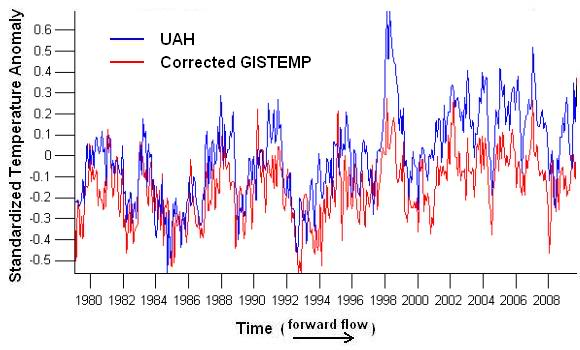
\includegraphics[scale=0.5]{invalid-corrected-gistemp.jpeg}}
}
\put(15,-15){Figure 1.0: UAH Satellite record vs. skewed GISTEMP readings.}
\end{picture}
\end{center}
\vspace{15 mm}

\begin{center} % Figures
\begin{picture}(320,235)
\put(0,0){
\setlength{\fboxsep}{20pt}
\setlength{\fboxrule}{1pt}
\fbox{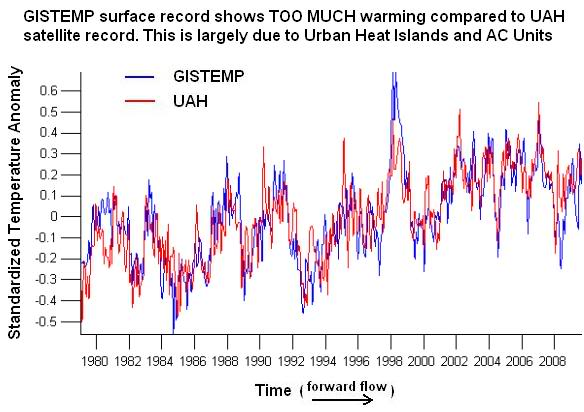
\includegraphics[scale=0.5]{initial-uah-gistemp.jpeg}}
}
\put(15,-15){Figure 1.1: UAH Satellite record vs. original GISTEMP readings.}
\end{picture}
\end{center}
\vspace{15 mm}

% TODO fix citation hansen 2010, is actually gistemp study
Many of these arguments relating to data are often either lacking professional citations, contain logical fallacies, or are misguided. It's true that when compared GISTEMP data is different from UAH Satellite records, however sensor data is expected to be different, and there is no evidence citing statistically significant variations in the two records. Pertaining to UHI, the GISTEMP study and other studies do their best to compensate for urban warm spots by spreading that anomaly across neighboring regions (Hansen 2010). Micro-site bias is also a valid issue, however misreading of individual station data are often discovered as outliers in the data set, and can be safely removed from final analysis. Attempts to discredit the organization or author tend to fall into feeble straw man arguments, a logical fallacy that misrepresents the opponents position.

% TODO elaborate on the additional studies
Many of the same arguments used against the GISTEMP study can be found trying to oppose other data sets like the UAH MSU, the RSS MSU, the HadCRUT3, the NCDC absolute, the NCDC anomaly, the CET, or the SIDC.
% http://junksciencearchive.com/MSU_Temps/Warming_Look.html

%This is an article criticizing the analysis created by NASA scientist, James Hansen. 
%http://en.wikipedia.org/wiki/James\_Hansen

%* straw man argument against james hansen

%* GISTEMP vs. UAH Satellite

%"Since 1979 satellites have been measuring the temperature of the lower atmosphere. GISTEMP is trying to measure the temperature of the surface." -

%"GISTEMP shows far more warming than the UAH satellite record."

%* Urban Heat Island Effect

%"Warmists will tell you there is no such thing as the urban heat island effect, but that's a complete strawman because their very own studies say there is an urban heat island effect. In fact they even try to correct for it in GISTEMP!

%As Blog Scientists we must assume they don't correct for UHI enough. Blog Science knows that GISTEMP is contaminated by UHI bias. In the following graph I correct GISTEMP for UHI by 0.01C/decade."

%Increase the bias by 0.01C/decade. Not enough of a difference so let's increase it by 0.05C/decade.

%What is the justification or factual reasoning behind arbitarily assuming what UHI compensation should be?

%The urban heat island effect is an observation that cities and urban developed areas are warmer than neighboring rural areas. By arbitrarily changing the UHI bias of the GISTEMP data, you are effectively changing the size and temperature of our global cities to make the data fit a less dramatic curve than it is as presented by GISS team.

%* Micro-Site Bias

%"tourists have left rubbish like barrels and boats lying around, items known to cause warming trends."

%"Warmists claim that the GISTEMP algorithm statistically detects and removes such significant biases from the record. But as Blog Scientists we assume otherwise."

%"Like with UHI bias the microsite bias must be somewhat large or else we would just be making a big deal about nothing! So I propose another correction of 0.05C, this time for microsite bias."

\section{Do Humans Significantly Effect The Environment?}
When arguing about climate change, some opponents will accept that temperatures have been increasing, or that global warming is happening, but they will deny that humans are a significant factor in causing the problem. Blame is shifted to natural or external causes that have been and will always be outside of our control.

% TODO fix bode citation, all names, pg #
% TODO comparison to pre-industrial co2 levels?
% TODO fix u w/ umluat in citation and sources
Thinking that we have no impact on the environment is untrue, and can be discredited in several ways using evidence. The typical evidence of human influence in climate change revolves around our CO2 and greenhouse gas emissions. The Carbon Dioxide Information Analysis Center, CDIAC, an office of the U.S. Department of Energy, estimates that we deposited upwards of 32 billion metric tons of carbon dioxide units into the atmosphere in the year 2008. (Boden 2010). We have ice core data that shows clear incrementing trends of CO2 averages (Inderm�hle 2008). We have records of CO2 content found in the air at the Mauna Loa observatory in Hawaii that show similar trends of growth in CO2 levels (Tans 2012). With evident growing levels of CO2 being found in our environment, we then hypothesize that radiation and energy will exit our atmospheric system at lower rates than in a system with less CO2. Our observations match this hypothesis, showing that higher CO2 levels in our environment are causing radiation to remain longer in our atmosphere. (Harries 2001) (Chen 2007). What this means is that humans significantly contribute to CO2 levels in the atomsphere, this CO2 remains in the atmosphere collecting radiation where it might normally escape, and this radiation is a cause of the warming we are seeing in our observed temperature data.
%http://www.skepticalscience.com/empirical-evidence-that-humans-are-causing-global-warming.html
%* We emit a shit ton of CO2
% http://cdiac.ornl.gov/trends/emis/overview_2006.html
% http://cdiac.ornl.gov/ftp/ndp030/global.1751_2008.ems
%8749 million metric tons of carbon
%To convert these estimates to units of carbon dioxide (CO2), simply multiply these estimates by 3.667

% ice core samples
% http://www.ncdc.noaa.gov/paleo/metadata/noaa-icecore-2419.html
%Taylor Dome - Carbon Dioxide Data
%needs a graph
% Mauna Loa CO2
% http://www.esrl.noaa.gov/gmd/ccgg/trends/
%* CO2 keeps warmth
%prevents radiation from leaving the atmosphere as easily. We can observe that this is the case
%http://www.nature.com/nature/journal/v410/n6826/abs/410355a0.html
% http://www.eumetsat.int/Home/Main/AboutEUMETSAT/Publications/ConferenceandWorkshopProceedings/2007/groups/cps/documents/document/pdf_conf_p50_s9_01_harries_v.pdf
%* The globe is accumulating heat
% http://www.agu.org/pubs/crossref/2009/2009JD012105.shtml

\section{The Politics Of Global Warming}
% TODO fix citation
In addition to data skeptics, and those who deny our impact in the environment are organizations and companies whose short term interests do not coincide with decreasing the use of fossil fuels. Fossil fuels are one of the leading causes of increased greenhouse gasses (CDIAC TODO).
% TODO see figure 2
% TODO fix citation
In 2011 spending for oil and gas related lobbying exceeded \$149 million dollars, and included contributors like Conoco Phillips, Shell, Exxon Mobil, Chevron, and the American Petroleum Institute. Yearly contributions, excluding incomplete data from 2012, show a clear trend of ever increased spending to lobby for the oil and gas industry (U.S. Office of Public Records).

% TODO cite
\begin{center} % Figures
\begin{picture}(320,235)
\put(0,0){
\setlength{\fboxsep}{20pt}
\setlength{\fboxrule}{1pt}
\fbox{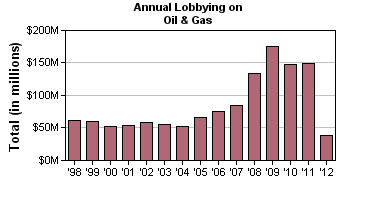
\includegraphics[scale=0.6]{oil-and-gas-lobbying-2012.png}}
}
\put(15,-15){Figure 2.0: Oil \& gas lobbying in the United States.}
\end{picture}
\end{center}
\vspace{15 mm}

% TODO fix year in citation
Though Exxon Mobil has never officially denied global warming, evidence has been shown that they have tried to discredit and add uncertainty to climate studies (``Smoke, Mirrors, \& Hot Air" 2007). This and companies that are similar have created road blocks of legislation towards improving the environment, and they have sought out short term financial gain without considering the long term cost of a degraded environment. They have profited off government subsidies, and are able to make a very large negative impact.

% TODO fix citation
% TODO vs. ? reconcile
% TODO awk.
Surprisingly, though, not all of these corporations take a negative stance towards a cleaner environment. Exxon Mobil's has released more recent updates showing them to support climate science and have an interest in helping (Mufson 2007). Other large oil companies want to help develop clean energy sources, and nuclear energy organizations have long sought out the elimination of fossil fuel usage.

When it comes to fossil fuels there is a lot of money riding along, and that money does a lot to hide the problems we face.

%funding, special interest groups, and pr campaigns have all been created by big money behind fossil fuels.
%exxonmobil publishing papers, and money to go against global warming

%nuclear energy, shell, and some others are for reducing green house gasses
% http://www.msnbc.msn.com/id/16593606/
% Exxon cuts ties to global warming skeptics
% Oil giant also in talks to look at curbing greenhouse gases

% http://www.ucsusa.org/assets/documents/global_warming/exxon_report.pdf
% http://www.exxonsecrets.org/html/listorganizations.php
% http://www.euronet.nl/users/e_wesker/ew@shell/API-prop.html
% http://www.washingtonpost.com/wp-dyn/content/article/2007/02/09/AR2007020902081.html
% Exxon Mobil Warming Up To Global Climate Issue


% http://thinkprogress.org/climate/2012/06/27/507710/as-exxon-ceo-calls-global-warmings-impacts-manageable-colorado-wildfires-shutter-climate-lab/?mobile=nc
% http://www.zmescience.com/ecology/climate-change-papers-exxon-mobil/

% http://www.garnautreview.org.au/2008-review.html
% http://webarchive.nationalarchives.gov.uk/+/http://www.hm-treasury.gov.uk/sternreview_index.htm

%governmental subsidies, throwing blame around, and simply spending money to move attention elsewhere

% oil & gas lobbying
% http://www.opensecrets.org/lobby/indusclient.php?id=E01&year=2011
% http://www.senate.gov/pagelayout/legislative/g_three_sections_with_teasers/lobbyingdisc.htm
%ConocoPhillips - \$20,557,043
%Royal Dutch Shell - \$14,790,000
%Exxon Mobil - \$12,730,000
%Chevron Corp - \$9,510,000
%American Petroleum Institute - \$8,640,000

%Total for Oil \& Gas: \$149,089,677
%Total Number of Clients Reported: 198	
%Total Number of Lobbyists Reported: 790	
%Total Number of Revolvers: 472 (59.7\%)
%oil-and-gas-lobbying-2011

%\subsection{From the source}
% http://pubs.giss.nasa.gov/docs/2010/2010_Hansen_etal.pdf
% http://www.agu.org/pubs/crossref/2010/2010RG000345.shtml
%"Global temperature is rising as fast in the
%past decade as in the prior 2 decades, despite year?to?year
%fluctuations associated with the El Ni�o?La Ni�a cycle of
%tropical ocean temperature. Record high global 12 month
%running mean temperature for the period with instrumental
%data was reached in 2010."

%\subsection{Summary}

%There are several sources for recorded temperature variations in the environment, but their data is skewed in favor of ring bells and raising alarm. We should be skeptical about the conclusions reached from these reports. The early data is too old to be accurate, and the present data has been misrepresented in several ways.

%Our process for measuring the data is bad. We aren't the cause of the increased temperatures, instead it's just something the earth does.
%Also stuff, and more stuff. I guess I'm just typing now with no point. Typing to type. Typing to make voise, and profess productivity. Busy to be busy. Looking around briefly while I avoid whatever the real issue is. I wonder what I'll do tomorrow, it is a holiday. 

%We avoid realizing the truth that global warming is not some event that is happening in the near distant future. It's an active process that is occurring right now. The CO2 in the atmosphere heats up the climate, which causes ice to melt which releases more greenhouse gasses. This additional release perpetuates the cycle. The atmosphere continues to heat itself up in an ongoing cycle that provides more and more damage over the course of time.

\section{Understanding What We Can Do}

The arguments against improving the environment and cutting fossil fuel consumption don't withstand critical peer review. When we understand that we're dealing with a real problem we can better set up goals and drive our society towards positive change. Our society is made up of individuals, all contributing and sharing. Though we can't always compete directly with the heavy financial interests and misinformation regarding climate degradation, we can improve our own impact.

Knowing that the main causes of CO2 and increased green house gasses in our environment come from the consumption of fossil fuels helps us pinpoint areas where we can improve the most.

\subsection{Vehicles}
% TODO fix uncited unfinished XX in text
% TODO telecommute if companies allow
% TODO lobby for better public/mass transport
% TODO clarify braking energy
We've become a commuter society, building vast transport infrastructure and making cars easy to purchase using convenient loan systems. Commuting daily takes it's toll on the environment. Commuters in the United States alone are shown to release XX amount of pollutants into the atmosphere a year. These days there is a lot we can do to cut down on driving. We can organize car-pools and ride-sharing that makes each vehicle more efficient by spreading the cost amongst a few. We can schedule telecommute days into our schedule where we can avoid driving and transportation altogether, relying on the speed and efficiency of wired communications over the internet. We can find and use public transportation systems more often. We can relocate to closer proximity and walk or bike as a commute. We can buy efficient engines that cleverly recycle braking energy into batteries. We can even push for robotic technology that will enable car sharing and computer controlled fuel efficiencies with our current vehicles. We can avoid vanity travel and airplane flights choosing more efficient methods of vacation. Our transportation infrastructure does not have to disappear and we don't need to cut ourselves off from movement, we just need moderation. We need to choose lifestyles where we aren't required to travel each and every day over long distances.

\subsection{Households}
Amongst our homes there are many things we can change to improve sustainability. Installing specialized solar cells can provide both energy, and heating in a self-sufficient manner. Small wind turbines can generate power in windy clear areas. We can even receive tax and utility credits by using these alternative energy sources. Our food consumption can improve by finding local farms who don't need to ship their produce and goods long distances, an unsustainable practice. Planting our own gardens and composting trash is cheap and efficient, requiring only time and effort to achieve. Avoiding the newest gadgets, and battery powered toys also helps to prevent expensive consumption, and polluting production of these devices.

\subsection{Speaking Up}
% TODO expand on last sentence
For every step we take to improve our individual carbon footprints, we must also share our knowledge and help others in equal part. Our climate problems were not created by uniquely identifiable offenders, but by groups of society over time. Likewise the solution does not lie in herculean efforts, but in cooperative and grassroots based teamwork. We must work together to dismiss the fallacies and misunderstandings that create opposition. Educating those around us on sustainable practices. Of course we should always speak up to our leaders and elected representatives, so they too have a vested interest in protecting the environment.

%\section{Proposal}
%\subsection{prompt}
%\subsection{draft}
%The purpose of my proposal is to curb environmental damage by
%suggesting alternative consumer practices and conservation of existing
%resources. 

%- Drive, fly, \& in general commute less. Fossil fuels make up one of
%  the largest contributers to environmental degradation
%- Seek out alternative energy sources in your own household. Personal
%  solar energy \& water heating. Gardening. Recycling trash, and
%  composting. 
%- Speak up to political and government leaders about energy and
%  environment related issues
%- Keep your older phones and computers longer in order to prevent
%  wasteful consumption.

%- include images
%- include citations
%\subsection{The Problem}
%\subsection{The Plan}
%\subsection{The Points}

\section{Conclusion}

There is no quick fix to solving climate issues. What we have ahead of us is an uphill battle, which will require tending on multiple fronts. We have to discourage reckless behavior relating to the environment we all share, and create new methods of thinking. By understanding what it is we are doing to damage the environment we can restrict these behaviors. By improving our acceptance of these facts we help to promote the larger problems we face. With effort many of us can lower our footprints in the environment leading to a positive impact at scale.

\begin{workscited}

\bibent
Boden, T.A., G. Marland, and R.J. Andres. 2010. \textit{Global, Regional, and National Fossil-Fuel CO2 Emissions.} Carbon Dioxide Information Analysis Center, Oak Ridge National Laboratory, U.S. Department of Energy, Oak Ridge, Tenn., U.S.A. doi 10.3334/CDIAC/00001\_V2010

\bibent
Chen, Claudine, John Harries, Helen Brindley, and Mark Ringer. ``Spectral Signatures of Climate Change in the Earth�s Infrared Spectrum between 1970 and 2006." \textit{EUMETSAT}. 2007. Web. 05 July 2012. $<$http://www.eumetsat.int/Home/Main/AboutEUMETSAT/Publications/ConferenceandWorkshopProceedings/2007/groups/cps/documents/document/pdf\_conf\_p50\_s9\_01\_harries\_v.pdf$>$.

\bibent
``Correcting GISTEMP." Web log post. Denial Depot. N.p., 8 Sept. 2009. Web. 05 July 2012. $<$http://denialdepot.blogspot.com/2009/11/correcting-gistemp.html$>$.

\bibent
Harries, John E., Helen E. Brindley, Pretty J. Sagoo, and Richard J. Bantges. ``Increases in Greenhouse Forcing Inferred from the Outgoing Longwave Radiation Spectra of the Earth in 1970 and 1997." \textit{Nature} 410 (2001): 355-57. Print.

\bibent
Inderm�hle A., Et. Al. 2008. \textit{Holocene carbon-cycle dynamics based on CO2 trapped in ice at Taylor Dome, Antarctica.} Nature 398:121-126.

\bibent
Mufson, Steven. ``Exxon Mobil Warming Up To Global Climate Issue." \textit{The Washington Post} 10 Feb. 2007: n. pag. 9 Feb. 2007. Web. 5 July 2012. $<$http://www.washingtonpost.com/wp-dyn/content/article/2007/02/09/AR2007020902081.html$>$.

\bibent
"Smoke, Mirrors, \& Hot Air." \textit{Union Of Concerned Scientists} (2007): Union Of Concerned Scientists. Jan. 2007. Web. 05 July 2012. $<$http://www.ucsusa.org/assets/documents/global\_warming/exxon\_report.pdf$>$.

\bibent
United States. Department of Commerce. National Oceanic \& Atmospheric Administration. \textit{Trends in Atmospheric Carbon Dioxide.} By Peter Tans and Ralph Keeling. N.p., n.d. Web. 05 July 2012. $<$http://www.esrl.noaa.gov/gmd/ccgg/trends/$>$.

\bibent
United States. Senate. Office of Public Records. \textit{Contributions Reporting.} Web. 05 July 2012. $<$http://www.senate.gov/pagelayout/legislative/g\_three\_sections\_with\_teasers/lobbyingdisc.htm$>$.

\end{workscited}
\end{mla}
\end{document}
